% Options for packages loaded elsewhere
\PassOptionsToPackage{unicode}{hyperref}
\PassOptionsToPackage{hyphens}{url}
%
\documentclass[12pt, letterpaper
]{article}
\usepackage{amsmath,amssymb}
\usepackage{lmodern}
\usepackage{iftex}
\ifPDFTeX
  \usepackage[T1]{fontenc}
  \usepackage[utf8]{inputenc}
  \usepackage{textcomp} % provide euro and other symbols
\else % if luatex or xetex
  \usepackage{unicode-math}
  \defaultfontfeatures{Scale=MatchLowercase}
  \defaultfontfeatures[\rmfamily]{Ligatures=TeX,Scale=1}
\fi
% Use upquote if available, for straight quotes in verbatim environments
\IfFileExists{upquote.sty}{\usepackage{upquote}}{}
\IfFileExists{microtype.sty}{% use microtype if available
  \usepackage[]{microtype}
  \UseMicrotypeSet[protrusion]{basicmath} % disable protrusion for tt fonts
}{}
\makeatletter
\@ifundefined{KOMAClassName}{% if non-KOMA class
  \IfFileExists{parskip.sty}{%
    \usepackage{parskip}
  }{% else
    \setlength{\parindent}{0pt}
    \setlength{\parskip}{6pt plus 2pt minus 1pt}}
}{% if KOMA class
  \KOMAoptions{parskip=half}}
\makeatother
\usepackage{xcolor}
\IfFileExists{xurl.sty}{\usepackage{xurl}}{} % add URL line breaks if available
\IfFileExists{bookmark.sty}{\usepackage{bookmark}}{\usepackage{hyperref}}
\hypersetup{
  hidelinks,
  pdfcreator={LaTeX via pandoc}}
\urlstyle{same} % disable monospaced font for URLs
\usepackage{graphicx}
\makeatletter
\def\maxwidth{\ifdim\Gin@nat@width>\linewidth\linewidth\else\Gin@nat@width\fi}
\def\maxheight{\ifdim\Gin@nat@height>\textheight\textheight\else\Gin@nat@height\fi}
\makeatother
% Scale images if necessary, so that they will not overflow the page
% margins by default, and it is still possible to overwrite the defaults
% using explicit options in \includegraphics[width, height, ...]{}
\setkeys{Gin}{width=\maxwidth,height=\maxheight,keepaspectratio}
% Set default figure placement to htbp
\makeatletter
\def\fps@figure{htbp}
\makeatother
\setlength{\emergencystretch}{3em} % prevent overfull lines
\providecommand{\tightlist}{%
  \setlength{\itemsep}{0pt}\setlength{\parskip}{0pt}}
\setcounter{secnumdepth}{-\maxdimen} % remove section numbering
\ifLuaTeX
  \usepackage{selnolig}  % disable illegal ligatures
\fi

\title{Multilayer Perceptron}
\author{PutinBoyZ}
\date{September 2022}

\begin{document}

\begin{titlepage}
  \maketitle
\end{titlepage}  

\textbf{Introduction}

Multilayer Perceptron (MLP) is a software designed to form and train neural network models to classify handwritten Latin letters. 

\textbf{Features and capabilities}

MLP app has thee main tabs:

\begin{itemize}
\item
  Testing: test trained neural network on a dataset
\item
  Training: train neural network on a dataset
\item
  Images: classify individual images (loaded or drawn)
\end{itemize}

In the settings panel user can change perceptron type, load and save current percepton, and chose datasets for training and testing.

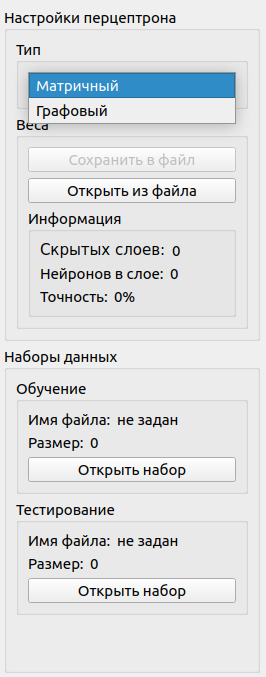
\includegraphics[width=4.72361in,height=3.25208in]{images/settings.png}

\textbf{Training}

To start using the program, user must load existing perceptron in the settings panel or train a new one.

To train new perceptron, user should:

\begin{enumerate}
    \item Open the training tab
    \item Choose peceptrons type and dataset for testing in settings panel
    \item Choose amount of hidden layers2-5, amount of epochs, and testing speed in training tab
    \item Press "Begin training" and wait
\end{enumerate}

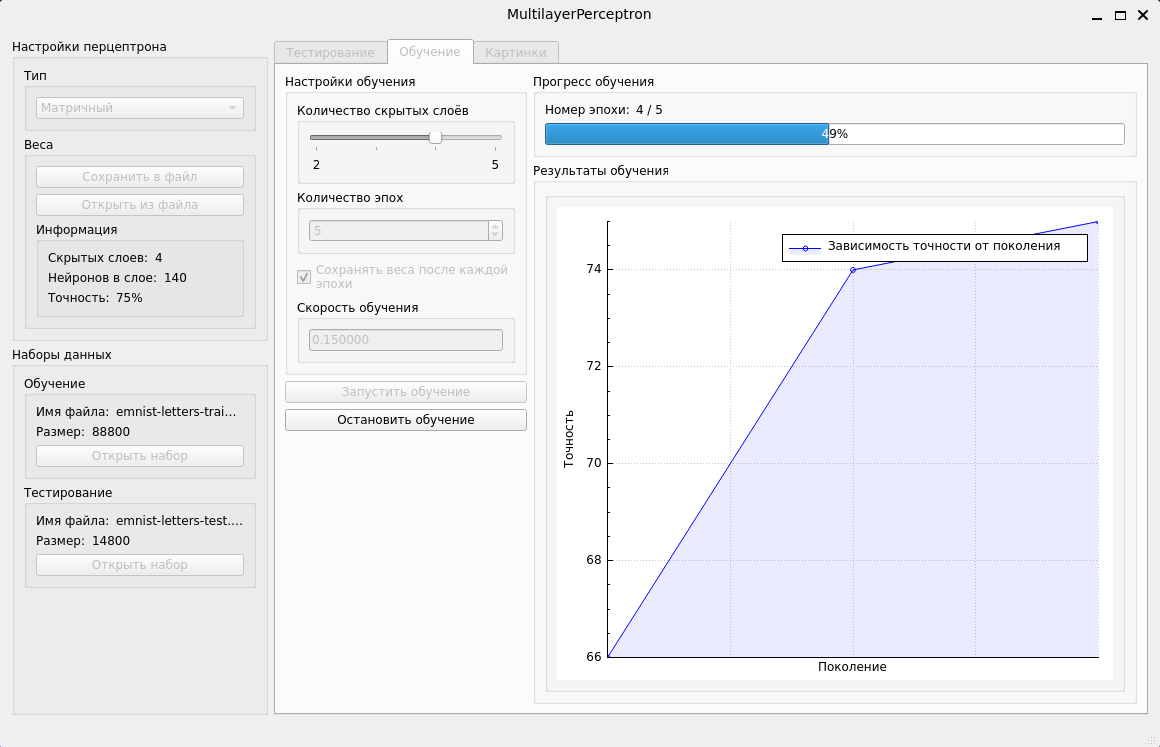
\includegraphics[width=4.72361in,height=3.25208in]{images/training.png}

After each epoch, information on this epochs error control values will be displayed.

\textbf{Testing}

After loading or training new perceptron, user can test in on the dataset in testing tab, or classify individual messages in images tab.

When testing is done an average accuracy, precision, recall, f-measure and total time spent on the experiment will be displayed on the screen.
Testing can be done with or without cross-validation. If cross-validation is on, results will be displayed for the best group.

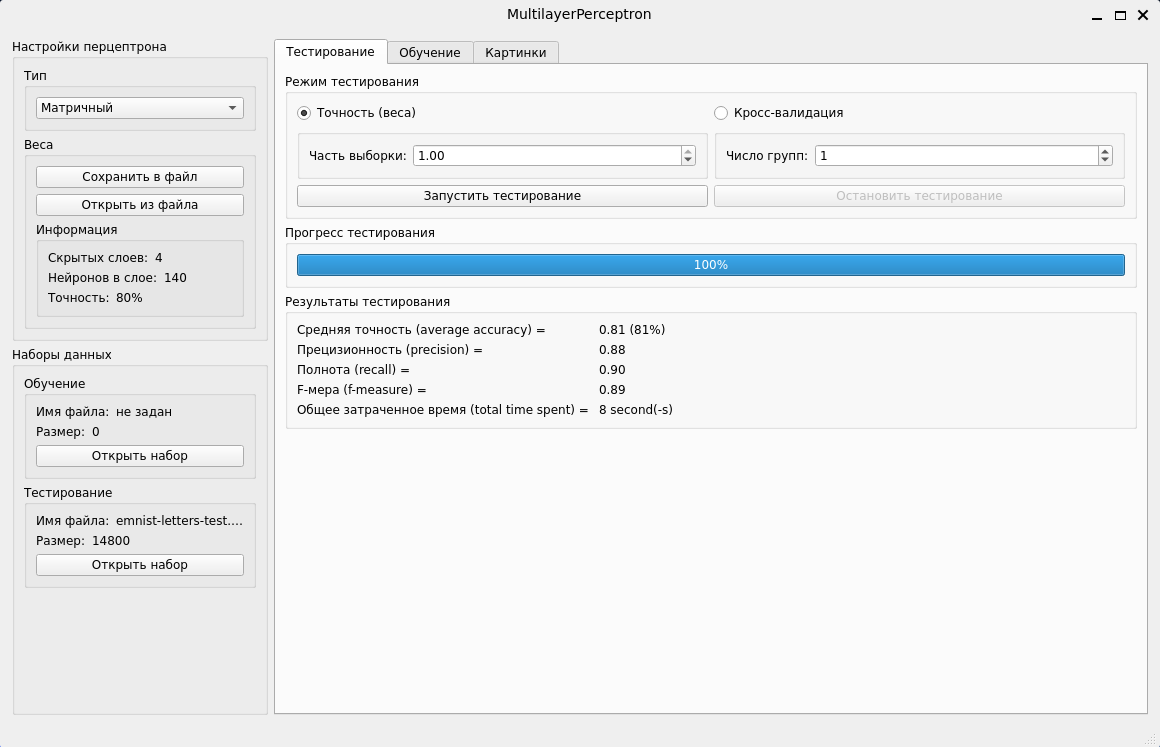
\includegraphics[width=4.72361in,height=3.25208in]{images/testing.png}

Images can be loaded or drawn by user.

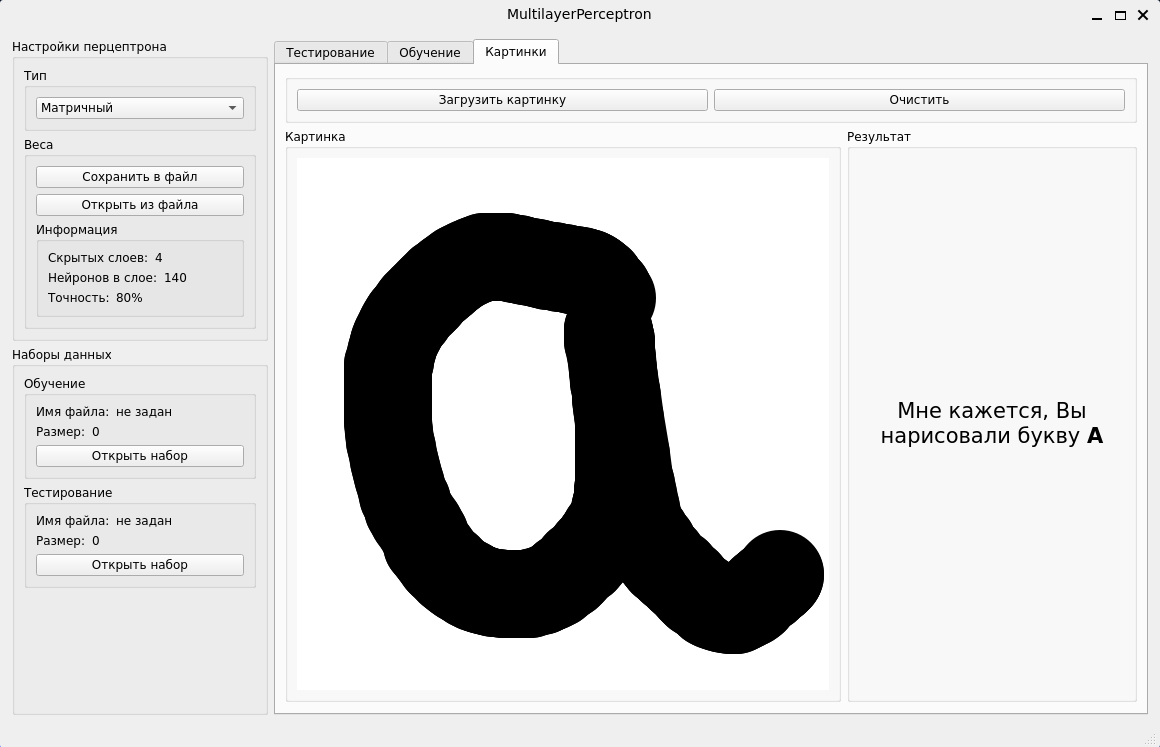
\includegraphics[width=4.72361in,height=3.25208in]{images/images.png}

\end{document}
